\subsection{Решения для рендеринга в реальном времени}
\label{sec:raycasting_splatting}

Как было выяснено в предыдущем разделе, для осуществления рендеринга требуются знания о свойствах среды во всех её точках. Эти данные задаются на обыкновенной воксельной сетке.

Для быстрой визуализации объемных данных удобно считать, что рассеивание отсутствует, так как из-за него возникают трудно отслеживаемый in-scattering. Если принять $\sigma_a=\sigma$, $\sigma_s=0$, уравнение \ref{eq:graphics_rte} упрощается до
%
\[
	\frac{\mathrm dL}{\mathrm dt} = -\sigma L + L_e.
\]
%
Решение уравнения приводится в работе \cite{max1995optical}, из которой
%
\begin{equation}
	\label{eq:int_rte_emm_abs}
	L(t) = L(0)e^{-\tau(t)} + \int_0^t L_e(s) e^{-\tau(s)} ds,
\end{equation}
%
\[
	\tau(t) = \int_0^t \sigma(s) ds.
\]

\begin{figure}[ht]
	\centering
	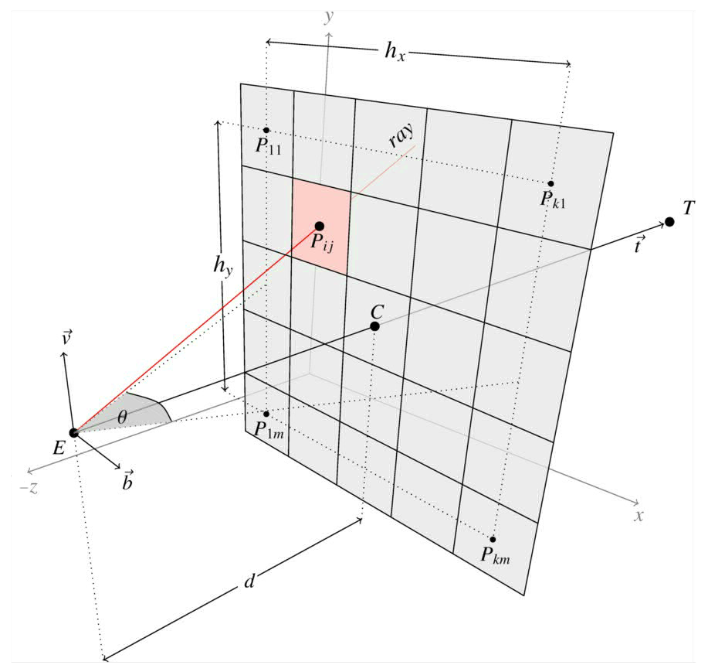
\includegraphics[width=0.5\textwidth]{assets/ray-casting.png}
	\caption{Пример испускания лучей через центры всех пикселей изображения (метод Ray Casting).}
	\label{fig:ray_casting}
\end{figure}

\textbf{Ray casting}. (рисунок \ref{fig:ray_casting}) Луч можно представить как
%
\[
	\mathrm r(t) = \mathrm o + t\mathrm d,
\]
%
где $\mathrm o$ - центр камеры, $\mathrm d$ - единичный вектор, соединяющий центр камеры и центр соответствующего пикселя. Первый метод численного решения уравнения \ref{eq:int_rte_emm_abs} заключатся в испускании лучей из камеры (наблюдателя) через каждый пиксель проективной плоскости. C использованием метода конечных разностей вдоль луча $r$ с шагом $\Delta t$ вычисляется приблизительный ответ. Оказывается удобным ввести непрозрачность
%
\begin{equation}
	\label{eq:rc_transparency}
	1 - \alpha_i = e^{-\sigma(i\Delta t)\Delta t},
\end{equation}
%
которую удобней просчитать заранее\footnote{Стоит держать в голове, что непрозрачность зависит от величины шага и при его изменении потребует пересчета.}, как это уже было сделано с помощью функции переноса. Формула аккумулирования цвета (её также называют альфа-блендингом) имеет вид:
%
\begin{align}
	\label{eq:alpha_blending1}
	C^i_\text{acc} &=
		C^{i-1}_\text{acc} +
		(1 - \alpha^{i-1}_\text{acc}) (\alpha_i c_i); \\
	\label{eq:alpha_blending2}
	\alpha^i_\text{acc} &=
		a^{i-1}_\text{acc} +
		(1-\alpha^{i-1}_\text{acc}) \alpha_i,
\end{align}
%
где $c_i, \alpha_i$ вычисляются в точке $\mathrm o + i\Delta t \mathrm d$.

\begin{figure}[ht]
	\centering
	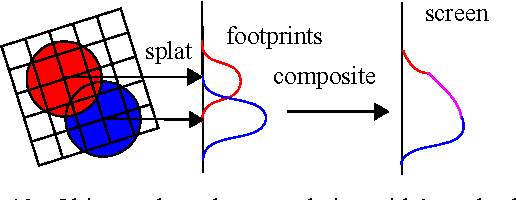
\includegraphics[width=0.5\textwidth]{assets/splatting.png}
	\caption{Ортографическая проекция гауссиан на экран (метод Splatting). Красним и синим здесь обозначены ядра, которыми заменены каждые воксели.}
	\label{fig:splatting}
\end{figure}

\textbf{Splatting}. (рисунок \ref{fig:splatting}) Вместо того, чтобы испускать лучи из камеры предлагается другой подход: проецировать воксели на камеру. В оригинальной статье, предложившей его \cite{westover1990footprint}, каждый воксель заменяется на функцию $h$ (ядро), что позволяет считать цвет и прозрачность каждой точки объема $(x, y, z)$ как
%
\[
	C(x, y, z) = \sum_i h(x-x_i, y-y_i, z-z_i) c_i,
\]
\[
	\alpha(x, y, z) = \sum_i h(x-x_i, y-y_i, z-z_i) \alpha_i.
\]
%
Суммирование ведется по всем вокселям, $(x_i, y_i, z_i), \alpha_i, c_i$ - координата центра, непрозрачность и цвет вокселя $i$ соответственно.

Конечно, у такого объема можно как и раньше вычислить изображение на экране методом ray casting, однако предлагается проецировать ядра на экран. В оригинальной статье модель проецирования --- ортографическая\footnote{Ортографическая проекция предполагает испускать лучи из центров каждого пикселя перпендикулярно плоскости изображения, в отличие от перспективной, где лучи испускаются из оптического центра камеры и проходят через центры пикселей.}, при этом не ограничивая общности лучи можно считать параллельнными $(0, 0, 1)$. Для ядра можно просчитать его влияние на луч, исходящий из $(x,y)$. Если просчитать все возможные лучи из плоскости $Oxy$, то получится двумерный отпечаток ядра
%
\begin{equation}
	h^i_\text{footprint} (x, y) = \int_{-\infty}^{+\infty} h(x-x_i, y-y_i, z-z_i) \mathrm dz.
	\label{eq:footprint}
\end{equation}
%
Непрозрачность и цвет каждого вокселя для текущего отрисовываемого пикселя пропорционально отпечатку. Учитывая удаленность центров ядер от плоскости, итоговое изображение можно получить по ранее выведенным формулам альфа-блендинга \ref{eq:alpha_blending1} и \ref{eq:alpha_blending2}.

Splatting с ядром Гаусса являются основоположниками 3D Gaussian Splatting, который подробно рассматривается в разделе \ref{sec:3dgs}.